\chapter{Test e valutazioni}\label{test-e-valutazioni}

In questo capitolo viene illustrata la metodologia adottata per testare
e validare il funzionamento del sistema di traduzione Text-to-SQL
progettato. Al fine di garantire l'oggettività e la coerenza dei test
prestazionali, la fase di sperimentazione ha previsto l'impiego di due
dei dataset di riferimento nel panorama internazionale per la
generazione di codice SQL: Spider e BIRD (Big
Bench for Large-scale Database Grounded Text-to-SQL Evaluation).

Ciascun dataset fornisce un corpus eterogeneo di interrogazioni in
linguaggio naturale correlate alle rispettive query di riferimento
(denominate gold queries), oltre agli schemi logici dei database
in formato JSON e a uno script di validazione automatico. Tali script
consentono di confrontare l'output della query predetta con quello della
query target, definendo un benchmark rigoroso per la valutazione delle
performance.

Il primo dataset, Spider, dispone di venti database distinti, reperiti
attraverso risorse accademiche, tutorial dedicati e portali online
specializzati, tra cui DatabaseAnswers e WikiSQL \cite{yu2019spiderlargescalehumanlabeleddataset}. La nomenclatura di
tabelle e colonne è stata preventivamente normalizzata (ad esempio,
trasmutando l'identificativo \texttt{stu\_id} in \texttt{student\_id})
per assicurare che i metadati risultassero auto-esplicativi; tale
accorgimento permette ai modelli linguistici di concentrarsi sul parsing
semantico anziché sulla decifrazione di abbreviazioni criptiche \cite{yu2019spiderlargescalehumanlabeleddataset}. Le 1034
richieste di input sono state generate manualmente da studenti di
informatica esperti in linguaggio SQL, escludendo l'uso di template
automatici al fine di preservare la naturalezza e la variabilità del
linguaggio umano \cite{yu2019spiderlargescalehumanlabeleddataset}. Le domande di Spider coprono i principali costrutti
SQL all'interno di ciascun pool di database e sono state concepite per
essere chiare ed univoche \cite{yu2019spiderlargescalehumanlabeleddataset}. Sono state deliberatamente escluse richieste
che imponessero il ricorso a conoscenze esterne al database o inferenze
basate sul senso comune \cite{yu2019spiderlargescalehumanlabeleddataset}. Per garantire la più alta qualità dell'input possibile, il
dataset è stato inoltre sottoposto a molteplici fasi di revisione e
validazione incrociata \cite{yu2019spiderlargescalehumanlabeleddataset}.

Il benchmark BIRD si discosta parzialmente dall'approccio precedente,
attingendo a scenari applicativi reali provenienti da piattaforme come
Kaggle o repository pubbliche di GitHub, andando a comporre un set di
dieci database complessi \cite{3666122.3667957}. Le 1534 richieste sono state generate tramite
un processo di crowdsourcing rigoroso strutturato secondo precisi
criteri di complessità logica, introducendo per la prima volta quesiti
che richiedono capacità di External Knowledge Reasoning
(ragionamento basato su conoscenza esterna) \cite{3666122.3667957}. Ogni singola domanda è
stata preventivamente testata per garantire che la corrispondente query
SQL di riferimento non restituisse un set di risultati nullo \cite{3666122.3667957}.

Entrambi i framework offrono metriche dedicate per verificare
l'accuratezza dei risultati. Per quanto riguarda Spider, l'obiettivo
primario risiede nel testare la capacità di un modello di generalizzare
su nuovi schemi relazionali e domini mai visti in fase di addestramento
(cross-domain evaluation), focalizzandosi sulla complessità
sintattica della query generata \cite{yu2019spiderlargescalehumanlabeleddataset}. La valutazione scompone
l'interrogazione nei suoi componenti principali (\texttt{SELECT},
\texttt{WHERE}, \texttt{GROUP\ BY}, ecc.), analizzandoli come insiemi
non ordinati di sotto-componenti al fine di gestire l'assenza di vincoli
sequenziali rigidi nel linguaggio SQL. Il giudizio algoritmico si
articola in tre metriche fondamentali: Component Matching, Exact
Matching e Hardness Criteria \cite{yu2019spiderlargescalehumanlabeleddataset}.

Il benchmark BIRD nasce invece con l'intento di superare i limiti
strutturali di Spider, introducendo database su larga scala (pari a 33,4
GB complessivi) caratterizzati da dati non normalizzati e affetti da
rumore di fondo, simulando fedelmente i contesti industriali reali \cite{3666122.3667957}. Di
conseguenza, i criteri di valutazione si evolvono verso una validazione
prettamente esecutiva, articolandosi in: Execution Accuracy (EX), Valid
Efficiency Score (VES) ed External Knowledge Reasoning\cite{3666122.3667957}.

La suite di test è stata eseguita su una selezione di Modelli
Linguistici ad Ampio Spettro (LLM) di ultima generazione, afferenti ai
principali provider del settore e ottimizzati per la generazione di
codice: \emph{GPT-4o}, \emph{GPT-5-mini}, \emph{Codestral (22B)},
\emph{CodeLlama (34B)}, \emph{SQLCoder (34B)} e \emph{Qwen3-Coder-Next}.

\section{Architettura del Sistema di
Testing}\label{architettura-del-sistema-di-testing}

Per condurre la campagna di test in modo efficiente, mitigando i tempi
morti legati alle latenze delle chiamate API esterne, è stata progettata
un'architettura software multithreading. Il sistema distribuisce il
carico computazionale istanziando un thread concorrente per ciascun
modello LLM configurato (\emph{Generator Thread}). Questo ecosistema
viene coordinato da un ulteriore thread concorrente dedicato al
monitoraggio (\emph{Printer Thread}). Tale parallelizzazione consente di
sottoporre simultaneamente lo stesso set di quesiti a tutti i modelli,
ottimizzando i tempi complessivi di esecuzione del benchmark.

Il processo d'ispezione si articola attraverso una sequenza
deterministica di fasi. All'avvio, il sistema acquisisce i parametri
operativi da riga di comando o, in subordine, tramite una procedura
guidata interattiva. L'utente definisce il dataset di riferimento
(Spider o BIRD), il database bersaglio e la modalità operativa del test,
discriminando tra l'approccio puramente testuale (\texttt{text}) e
quello basato sulla connessione diretta al DBMS (\texttt{db\_conn}).
L'architettura applica il principio della programmazione orientata agli
oggetti mediante la classe astratta \texttt{BaseDataset}. Questa
definisce l'interfaccia e i metodi standard che le sottoclassi concrete
\texttt{SpiderDataset} e \texttt{BirdDataset} sono obbligate a
implementare. All'atto dell'istanziazione, la sottoclasse selezionata
popola le proprie strutture dati caricando i file descrittivi del
benchmark: il file \texttt{dev.json} (contenente i prompt utente), il
file \texttt{tables.json} (contenente le definizioni degli schemi) e i
puntatori ai moduli di computazione delle metriche ufficiali. Il sistema
esegue una routine di sanificazione ambientale, azzerando le directory
temporanee (\texttt{tmp}) e predisponendo la struttura delle cartelle
deputate ad accogliere i log e i report intermedi. Contestualmente,
viene inizializzato l'oggetto \texttt{Schema} e agganciato al
corrispondente \texttt{SchemaStore}. Un elemento critico del design
software riguarda la persistenza dei fallimenti. Poiché tutti i
\emph{Generator Threads} accedono contemporaneamente alla risorsa
condivisa \texttt{QueryStore} per registrare e consultare le query
errate, si rende necessario prevenire fenomeni di race condition.
Il problema è stato risolto implementando la classe
\texttt{ThreadSafeQueryStore}, una derivazione di \texttt{QueryStore}
che incapsula le primitive di scrittura e lettura all'interno di un
meccanismo di mutua esclusione (Thread Lock).

Una volta avviati, i \emph{Generator Threads} istanziano dinamicamente
un'apposita componente \texttt{QueryOrchestrator}, configurata con i
parametri del modello e del client specifici del thread.
Successivamente, il thread itera sul set di quesiti in linguaggio
naturale estratti dal dataset, invocando il metodo \texttt{generation}.

I risultati d'inferenza vengono incapsulati in un oggetto
\texttt{QuerySession}. Qualora l'orchestratore concluda l'elaborazione
con uno stato di successo (\texttt{SUCCESS}), la sessione viene
inoltrata al modulo di valutazione del dataset per subirne il giudizio
assoluto. Al fine di garantire l'affidabilità dei log, il thread
implementa una gestione delle eccezioni di runtime: il
sollevamento di un \texttt{TimeoutError} (dovuto a saturazione del
canale o latenza del provider) comporta la classificazione esplicita
dello stato come \texttt{TIMEOUT\_ERROR}, mentre le anomalie impreviste
vengono mappate sotto la categoria generale \texttt{RUNTIME\_ERROR}. In
entrambi i casi, il sistema genera un oggetto \texttt{RequestResult}
contrassegnato da un flag di fallimento, impedendo il blocco dei thread
paralleli.

Il \emph{Printer Thread} opera in regime di ascolto passivo su una coda
sincronizzata (\texttt{result\_queue}). Man mano che i thread di
generazione depositano i rispettivi oggetti \texttt{RequestResult}, il
coordinatore aggiorna una matrice di stato interna
(\texttt{results\_by\_index}) e notifica l'avanzamento su terminale
standard tramite la funzione \texttt{print\_model\_progress}. Al
completamento di ciascun quesito da parte di tutti i modelli, il sistema
scrive un file testuale intermedio, minimizzando il rischio di perdita
dei dati in caso di interruzione accidentale. Al termine della sessione
globale, il thread consolida la matrice dei risultati generando il
report conclusivo aggregato per metriche temporali, accuratezza ed
efficacia dei metodi di raffinamento.

La verifica dell'accuratezza delle query SQL prodotte rappresenta un
compito complesso, poiché una medesima richiesta semantica può essere
espressa attraverso costrutti sintattici differenti ma logicamente
equivalenti. I validatori standard mostrano spesso una rigidità
eccessiva, portando alla luce numerosi ``falsi negativi'': query
considerate errate a causa di discrepanze formali marginali, come
l'ordine delle colonne o la loro rinominazione. Per ovviare a tali
limiti, è stato architettato un framework di valutazione stratificato su
tre livelli sequenziali.

Il primo livello si interfaccia direttamente con l'infrastruttura di
verifica ufficiale fornita a corredo dei dataset mediante il metodo
\texttt{dataset\_evaluation}. Sia per Spider che per BIRD, l'ispezione
avviene invocando un sottoprocesso isolato di sistema che esegue la
query predetta sull'ambiente database nativo. L'output del sottoprocesso
viene catturato e strutturato in un oggetto \texttt{OfficialEvalReport}.
La metrica cardinale estratta è la \emph{Execution Accuracy}
(\texttt{execution\_accuracy}), un indicatore numerico espresso come
float (\(1.0\) in caso di perfetta corrispondenza tra i record estratti
dalla query predetta e quelli della \emph{gold query}, \(0.0\) in caso
di disallineamento o errore strutturale).

I validatori ufficiali dei dataset mostrano un'elevata suscettibilità a
variazioni non sostanziali, quali l'ordinamento delle righe o la
nomenclatura interna delle colonne, generando talvolta fenomeni di falso
negativo. Il secondo livello d'ispezione interviene per mitigare tale
rigidità effettuando un confronto diretto e controllato dei set di dati
risultanti. Il sistema esegue una routine di normalizzazione dei tipi di
dato (uniformando formati di stringhe, date e floating-point) e analizza
i risultati secondo regole euristiche:

\begin{itemize}
\item
  \textbf{Exact Match:} Identità assoluta dei set di record estratti,
  che convalida la query restituendo il valore
  \code{ComparisonResult.EXACT_MATCH}.
\item
  \textbf{Row Count Mismatch:} Discrepanza quantitativa nel numero di
  tuple restituite (\code{ComparisonResult.ROW_COUNT_MISMATCH}).
\item
  \textbf{Sottoinsieme di Colonne:} Verifica algebrica volta ad
  accertare se l'anomalia sia limitata all'inclusione o proiezione di
  colonne spurie, mantenendo l'integrità del nucleo informativo
  richiesto.
\end{itemize}

Qualora la query fallisca le verifiche deterministiche precedenti, il
framework demanda il giudizio definitivo a un modello linguistico d'alto
livello configurato come arbitro semantico (\texttt{\_run\_llm\_judge}).
Il giudice finale altro non è che un LLM scelto appositamente per le sue 
notevoli conoscenze linguistiche e la sua capacità di ragionamento logico, 
nello specifico si tratta di Qwen3-Coder-Next.
Sfruttando la classe \texttt{PromptBuilder}, viene formulato un prompt
che espone la \emph{gold query} con il rispettivo set di dati atteso, e
la query generata con il suo specifico output esecutivo \ref{lst:prompt_judge}. Il modello ha
il compito di trascendere le differenze sintattiche superficiali per
valutare se la logica della query predetta rispetti l'intento
informativo dell'utente. L'output dell'oracolo viene strutturato in un
dizionario standardizzato contenente un verdetto
(\texttt{verdict:~correct/incorrect}) e una stringa motivazionale
dettagliata (\texttt{reason}) in caso di esito negativo.

L'intero ciclo si conclude con la restituzione di un oggetto
\texttt{EvaluationResult}, il quale mappa in modo trasparente lo storico
dei tentativi, le query coinvolte e i dettagli analitici emessi dai tre
livelli di controllo, offrendo una base dati robusta per l'analisi
comparativa delle prestazioni dei singoli modelli.

\begin{figure}
  \centering
    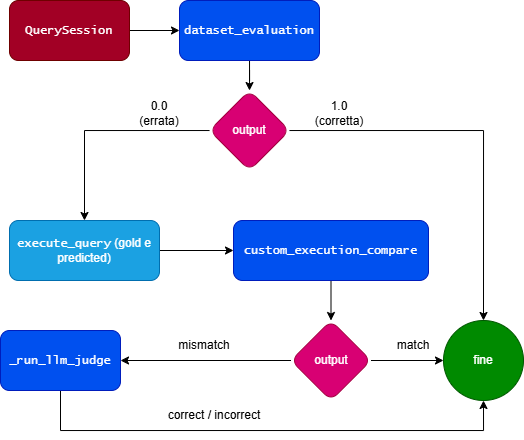
\includegraphics[width=0.60\textwidth]{immagini/workflows/dataset_evaluation.png}
  \caption{Flusso di valutazione della query SQL con il dataset.}
\end{figure}

\section{Fase di analisi}\label{fase-di-analisi}

Al fine di garantire il rigore scientifico e la perfetta riproducibilità
della fase di valutazione sperimentale, è stato sviluppato un modulo
software dedicato alla gestione, standardizzazione ed elaborazione
statistica dei tracciati di esecuzione prodotti dai \emph{Large Language
Models}. Il componente, implementato nello script
\texttt{summarize\_models.py}, agisce come un motore di aggregazione
cross-model, operando a partire dai log strutturati in formato
JSON memorizzati al termine delle sessioni di test per ciascun database
del benchmark.

Il modulo implementa un'architettura di calcolo che mappa i risultati
empirici secondo le due distinte modalità operative di interazione con
lo schema relazionale introdotte precedentemente: la modalità connessa
(\texttt{db\_conn}), basata sull'ispezione dinamica e sull'estrazione
nativa dei metadati dal DBMS, e la modalità puramente testuale
(\texttt{text}), vincolata alla fornitura statica delle istruzioni DDL
nel prompt dell'LLM.

L'analisi quantitativa si articola su una matrice di vettori e variabili
strutturate per valutare la resilienza, l'efficienza e l'accuratezza
semantica dell'intero sistema. I parametri cardinali e le metriche
integrate all'interno del report di sintesi sono così definiti:

\begin{itemize}
\item
  \textbf{Dataset e Database:} identificativi univoci del dominio
  applicativo e dell'istanza relazionale sottoposta a benchmarking.
\item
  \textbf{Metadati Strutturali (\(N_t\), \(N_c\)):} rispettivamente, il
  numero di entità relazionali (tabelle, \(N_t\)) e il numero
  complessivo di attributi (colonne, \(N_c\)) che compongono lo schema
  target.
\item
  \textbf{Densità Relazionale (\(D_r\)):} rapporto metrico espresso come
  \(D_r = N_c / N_t\), indicativo del livello medio di capienza
  informativa e di ramificazione delle tabelle.
\item
  \textbf{Requests:} il volume campionario totale di query espresse in
  linguaggio naturale sottoposte al sistema per lo specifico schema.
\item
  \textbf{Triplet Score:} rappresentazione vettoriale della
  distribuzione della complessità delle query, ripartita in tre
  macro-classi discrete sulla base di una soglia empirica determinata
  dal numero di costrutti logici rilevati:
\end{itemize}

\[
\text{Complessità} = 
\begin{cases} 
\text{Bassa (Low)}, & \text{se Score} \leq 3 \\ 
\text{Media (Medium)}, & \text{se } 3 < \text{Score} \leq 6 \\ 
\text{Alta (High)}, & \text{se Score} > 6 
\end{cases}
\]

\begin{itemize}
\item
  \textbf{Avg Query Complexity (\(Q\)):} media aritmetica del vettore
  dei punteggi di complessità intrinseca associati a ciascuna richiesta
  utente all'interno del database.
\item
  \textbf{Complexity Score (\(C_{db}\)):} indice normalizzato della
  complessità architetturale globale del database, derivato combinando
  la complessità sintattica delle richieste con la densità dello schema
  relazionale.
\item
  \textbf{Success Rate:} frequenza relativa dei successi del modello
  (calcolata distintamente per le modalità \texttt{db\_conn} e
  \texttt{text}), espressa come rapporto percentuale tra le query
  validate come corrette dall'infrastruttura di controllo e i tentativi
  totali eseguiti nell'ambiente operativo.
\end{itemize}

Per ponderare in modo oggettivo le performance dei singoli modelli in
base alla difficoltà intrinseca del contesto relazionale, il modulo
implementa una funzione di normalizzazione della complessità del
database. Definita \(S = N_c / N_t\) la densità dello schema corrente e
\(S_{\max}\) il valore massimo registrato nell'intero benchmark, il
componente calcola il punteggio finale di complessità del database
(\(C_{db}\)) mediante la seguente equazione lineare:

\[
C_{db} = Q \cdot \left(1 + 0.25 \cdot \frac{S}{S_{\max}}\right)
\]

Il modello matematico applicato assicura che l'architettura dello schema
relazionale agisca come fattore moltiplicativo di penalizzazione (fino a
un massimo del 25\%) sulla complessità media delle query (\(Q\)),
riflettendo l'effettivo overhead cognitivo imposto ai modelli LLM
dalla presenza di schemi estesi e densamente popolati.

Contestualmente, per l'analisi approfondita dei casi di insuccesso, lo
script esegue una categorizzazione deterministica degli output non
conformi, isolando tre macro-classi di errore:

\begin{enumerate}
\def\labelenumi{\arabic{enumi}.}
\item
  \textbf{Syntax Error:} inabilità del modello a generare un costrutto
  SQL sintatticamente valido per il dialetto di riferimento,
  intercettato formalmente in fase di parsing o validazione astratta.
\item
  \textbf{Runtime Error:} eccezioni sollevate direttamente in fase di
  esecuzione sul DBMS (quali riferimenti ad attributi o tabelle
  inesistenti e violazioni dei vincoli di integrità referenziale).
\item
  \textbf{Incorrect (Semantic Error):} query eseguite correttamente dal
  motore di database senza sollevare eccezioni, ma caratterizzate da un
  disallineamento semantico (esito logico e tuple estratte divergenti)
  rispetto alla ground truth di valutazione.
\end{enumerate}

Infine, per comprendere i fattori esogeni ed endogeni che governano il
decadimento prestazionale o la robustezza dei modelli, lo script esegue
un'analisi inferenziale calcolando i coefficienti di correlazione
lineare di Pearson (\(\rho\)) e di correlazione per ranghi di Spearman
(\(r_s\)). L'algoritmo allinea i vettori delle metriche continue (es.
numero di tentativi effettuati, complessità normalizzata della query)
con i vettori dicotomici associati all'esito della sessione
(\(Y \in \{0, 1\}\), dove \(1\) indica il successo e \(0\) il
fallimento).

Il \emph{Coefficiente di Pearson} (\(\rho\)) viene impiegato per
misurare l'intensità di una relazione lineare tra la metrica
indipendente e la probabilità di successo dell'output, mentre il
\emph{Coefficiente di Spearman} (\(r_s\)) viene applicato per catturare
relazioni monotoniche non strettamente lineari, configurandosi come un
indicatore robusto in presenza di distribuzioni non parametriche o
fortemente sbilanciate.

Ciascun coefficiente viene validato mediante il calcolo del rispettivo
valore di significatività (\emph{p-value}). Il sistema rigetta l'ipotesi
nulla (\(H_0\): assenza di correlazione statistica) impostando un
livello di significatività alfa standard \(\alpha = 0.05\). Qualora uno
dei vettori presenti con varianza nulla, tipica presenza di una
costanza assoluta dei successi o dei fallimenti per un determinato
modello, l'algoritmo contrassegna il coefficiente come \emph{Non
Rilevabile} (ND), prevenendo anomalie computazionali e terminazioni
anomale derivanti dalla divisione per zero in fase di calcolo della
covarianza.

\subsection{Analisi Macro-Livello dei
Database}\label{analisi-macro-livello-dei-database}

Al fine di caratterizzare la robustezza e la resilienza del sistema
Text-to-SQL sviluppato, la \textbf{Tabella \ref{sec:tabella_database_summary}} riassume le metriche
strutturali e i tassi di successo globali (cross-model)
registrati sui 30 database facenti parte dei benchmark \emph{Spider} e
\emph{BIRD}. L'indagine a macro-livello permette di isolare l'impatto
combinato della complessità dello schema relazionale e della complessità
intrinseca delle query sul \emph{Success Rate} complessivo, evidenziando
eventuali scostamenti tra la modalità statica basata su prompt
testuale (\texttt{Success\ Rate\ text}) e la modalità dinamica guidata
dalla connessione nativa al DBMS (\texttt{Success\ Rate\ db\_conn}).

Dall'analisi sistematica del dataset emergono contesti applicativi in
cui i modelli dimostrano di essere in grado di fornire risposte corrette, supportata
da schemi relazionali compatti e richieste utente a bassa complessità
sintattica.

Il database \textbf{\texttt{poker\_player}} (\emph{Spider}) rappresenta
il punto di massimo successo per l'intero sistema, registrando un
\texttt{Success\ Rate\ db\_conn} del 94,58\% e un
\texttt{Success\ Rate\ text} del 72,92\% (Tabella \ref{sec:tabella_database_summary}). Tale
comportamento è strutturalmente giustificata da fattori architetturali
minimali: un numero di tabelle pari a \(N_t = 2\), una densità
relazionale controllata (\(D_r = 5,5\)) e, in particolare, l'indice di
complessità delle query più basso registrato nel campione
(\(\text{Avg Query Complexity} = 1,95\)). La distribuzione del
corrispondente \emph{Triplet Score} risulta infatti fortemente
polarizzata verso compiti elementari (32 query \emph{Low}, 8 \emph{Medium},
0 \emph{High}).

Analogamente, i database \textbf{\texttt{orchestra}} (\(89,58\%\) in
\texttt{db\_conn}), \textbf{\texttt{singer}} (\(90,56\%\) in
\texttt{db\_conn}) ed \textbf{\texttt{employee\_hire\_evaluation}}
(\(88,60\%\) in \texttt{db\_conn}) fanno intuire la tendenza per cui la
combinazione di schemi ridotti (\(N_t \le 4\)) e la sostanziale assenza
di query ad alta complessità nel \emph{Triplet Score} consente ai
modelli di convergere efficacemente verso la struttura SQL corretta
(Tabella \ref{sec:tabella_database_summary}). In questi domini, lo sforzo di astrazione semantica
richiesto è minimo, riducendo le probabilità di errore nell'allineamento
tra le entità relazionali.

Una dettagliata e successiva attività di audit condotta sui log
di sistema ha tuttavia fatto emergere una criticità sistematica,
parzialmente esogena rispetto alla complessità strutturale finora
discussa. Si è osservato che, persino in domini caratterizzati da un
contenuto numero di entità relazionali e da richieste utente
sintatticamente elementari, i modelli incorrono in fallimenti ripetuti a
causa dell'istanza dei dati e, nello specifico, delle operazioni di
filtraggio stringa nella clausola \texttt{WHERE}.

Quando la risoluzione del quesito in linguaggio naturale richiede
l'applicazione di predicati operanti su attributi di tipo
\texttt{VARCHAR} o \texttt{TEXT}, l'esatta stringa letterale (il
valore del record) non viene quasi mai esplicitata nella
consegna, né risulta deducibile dalla sola semantica dei metadati. In
questo modo i Large Language Models si trovano costretti a formulare
tentativi di computazione alla cieca. Tale dinamica innesca loop di
raffinamento iterativo infruttuosi che, nella maggior parte delle
istanze, determinano il definitivo fallimento della query per
disallineamento rispetto alla ground truth, pur mantenendo una
correttezza formale sotto il profilo sintattico.

Sul versante opposto, i decrementi prestazionali più severi si
concentrano spesso all'interno del sotto-insieme appartenente
al benchmark \emph{BIRD}, storicamente noto per presentare sfide più
vicine a scenari di produzione reali in termini di volume informativo e
ambiguità del linguaggio naturale.

Il caso più critico è rappresentato dal database
\textbf{\texttt{thrombosis\_prediction}}, il quale crolla a un tasso di
successo marginale del 2,25\% in modalità \texttt{text},
recuperando parzialmente fino al 10,63\% in modalità
\texttt{db\_conn} (Tabella \ref{sec:tabella_database_summary}). Nonostante lo schema presenti un numero
ridotto di tabelle (\(N_t = 3\)), esso mostra una densità relazionale
critica, con una media di 21,33 colonne per tabella (64
attributi complessivi) e un elevato \emph{Complexity Score} (3,87). La
presenza di un numero massivo di attributi satura la finestra di
contesto dei modelli in modalità \texttt{text}, innescando
fenomeni di allucinazione o disallineamento semantico nella selezione
dei campi.

Altrettanto complessi si rivelano i domini
\textbf{\texttt{california\_schools}} (\texttt{db\_conn} al 23,78\%) e
\textbf{\texttt{card\_games}} (\texttt{db\_conn} al 27,14\%) (Tabella
\ref{sec:tabella_database_summary}). In quest'ultimo scenario, l'overload informativo è guidato dalla
scala assoluta dello schema relazionale, caratterizzato da 115
colonne totali distribuite su 6 tabelle. Pur mantenendo una complessità
media delle query relativamente contenuta (2,25), la vastità del
catalogo dati circostante disorienta l'euristica di join e di proiezione
dei Large Language Models.

Un comportamento peculiare si osserva in
\textbf{\texttt{debit\_card\_specializing}} e
\textbf{\texttt{financial}}, i cui tassi in modalità \texttt{db\_conn}
si attestano rispettivamente al 19,79\% e 15,88\% (Tabella \ref{sec:tabella_database_summary}). In
questo caso, il principale fattore penalizzante non è ascrivibile allo
schema, bensì all'elevata complessità intrinseca delle richieste:
registrando un valore di \texttt{Avg\ Query\ Complexity} rispettivamente
di 5,05 e 4,64, le distribuzioni dei loro
\emph{Triplet Score} mostrano una netta prevalenza di query classificate
come \emph{Medium} e \emph{High}.

Il trend macroscopico più rilevante e matematicamente costante
rintracciabile nei dati è l'ampio delta prestazionale a favore della
modalità basata su connessione attiva al database (\texttt{db\_conn})
rispetto a quella puramente testuale (\texttt{text}).

Come evidenziato dall'andamento complessivo dei test, il passaggio dalla
modalità \texttt{text} alla modalità \texttt{db\_conn} genera un
incremento sistematico del \emph{Success Rate} su tutte le istanze
campionarie, con guadagni netti che superano frequentemente i
30-40 punti percentuali. Si vedano, a titolo esemplificativo, i
seguenti casi emblematici (Tabella \ref{sec:tabella_database_summary}):

\begin{itemize}
\item
  \textbf{\texttt{course\_teach}}: evidenzia una transizione da un
  iniziale 43,89\% (\texttt{text}) a un 78,33\%
  (\texttt{db\_conn}) {[}\(\Delta = +34,44\%\){]}.
\item
  \textbf{\texttt{cre\_Doc\_Template\_Mgt}}: si eleva dal 38,89\% a un
  78,17\% {[}\(\Delta = +39,28\%\){]}.
\item
  \textbf{\texttt{museum\_visit}}: sperimenta un netto incremento dal
  49,07\% a un 87,96\% {[}\(\Delta = +38,89\%\){]}.
\end{itemize}

Questo comportamento indica l'utilità della gestione dinamica del database 
da parte dell'orchestratore. Nella modalità \texttt{text},
l'immissione statica delle definizioni DDL nel prompt espone il modello
a un rumore informativo costante e all'incapacità di risolvere i tipi di
dato o i vincoli di integrità in tempo reale. Al contrario,
l'architettura \texttt{db\_conn} opera come un efficace vincolo
euristico esterno: l'estrazione mirata dei metadati, la validazione
dinamica del dialetto SQL e la facoltà di interrogare i cataloghi del
DBMS forniscono al framework di generazione una consapevolezza
contestuale. Questa sinergia mitiga le eccezioni a runtime e
gli errori di sintassi, stabilizzando le performance anche a fronte di
database caratterizzati da elevati indici di complessità.

%%%%%%%%%%%%%%%%%%%%%%%%%%%%%%%%%% db_successes %%%%%%%%%%%%%%%%%%%%%%%%%%%%%%%%%%%

\begin{figure}[htbp]
  \centering
  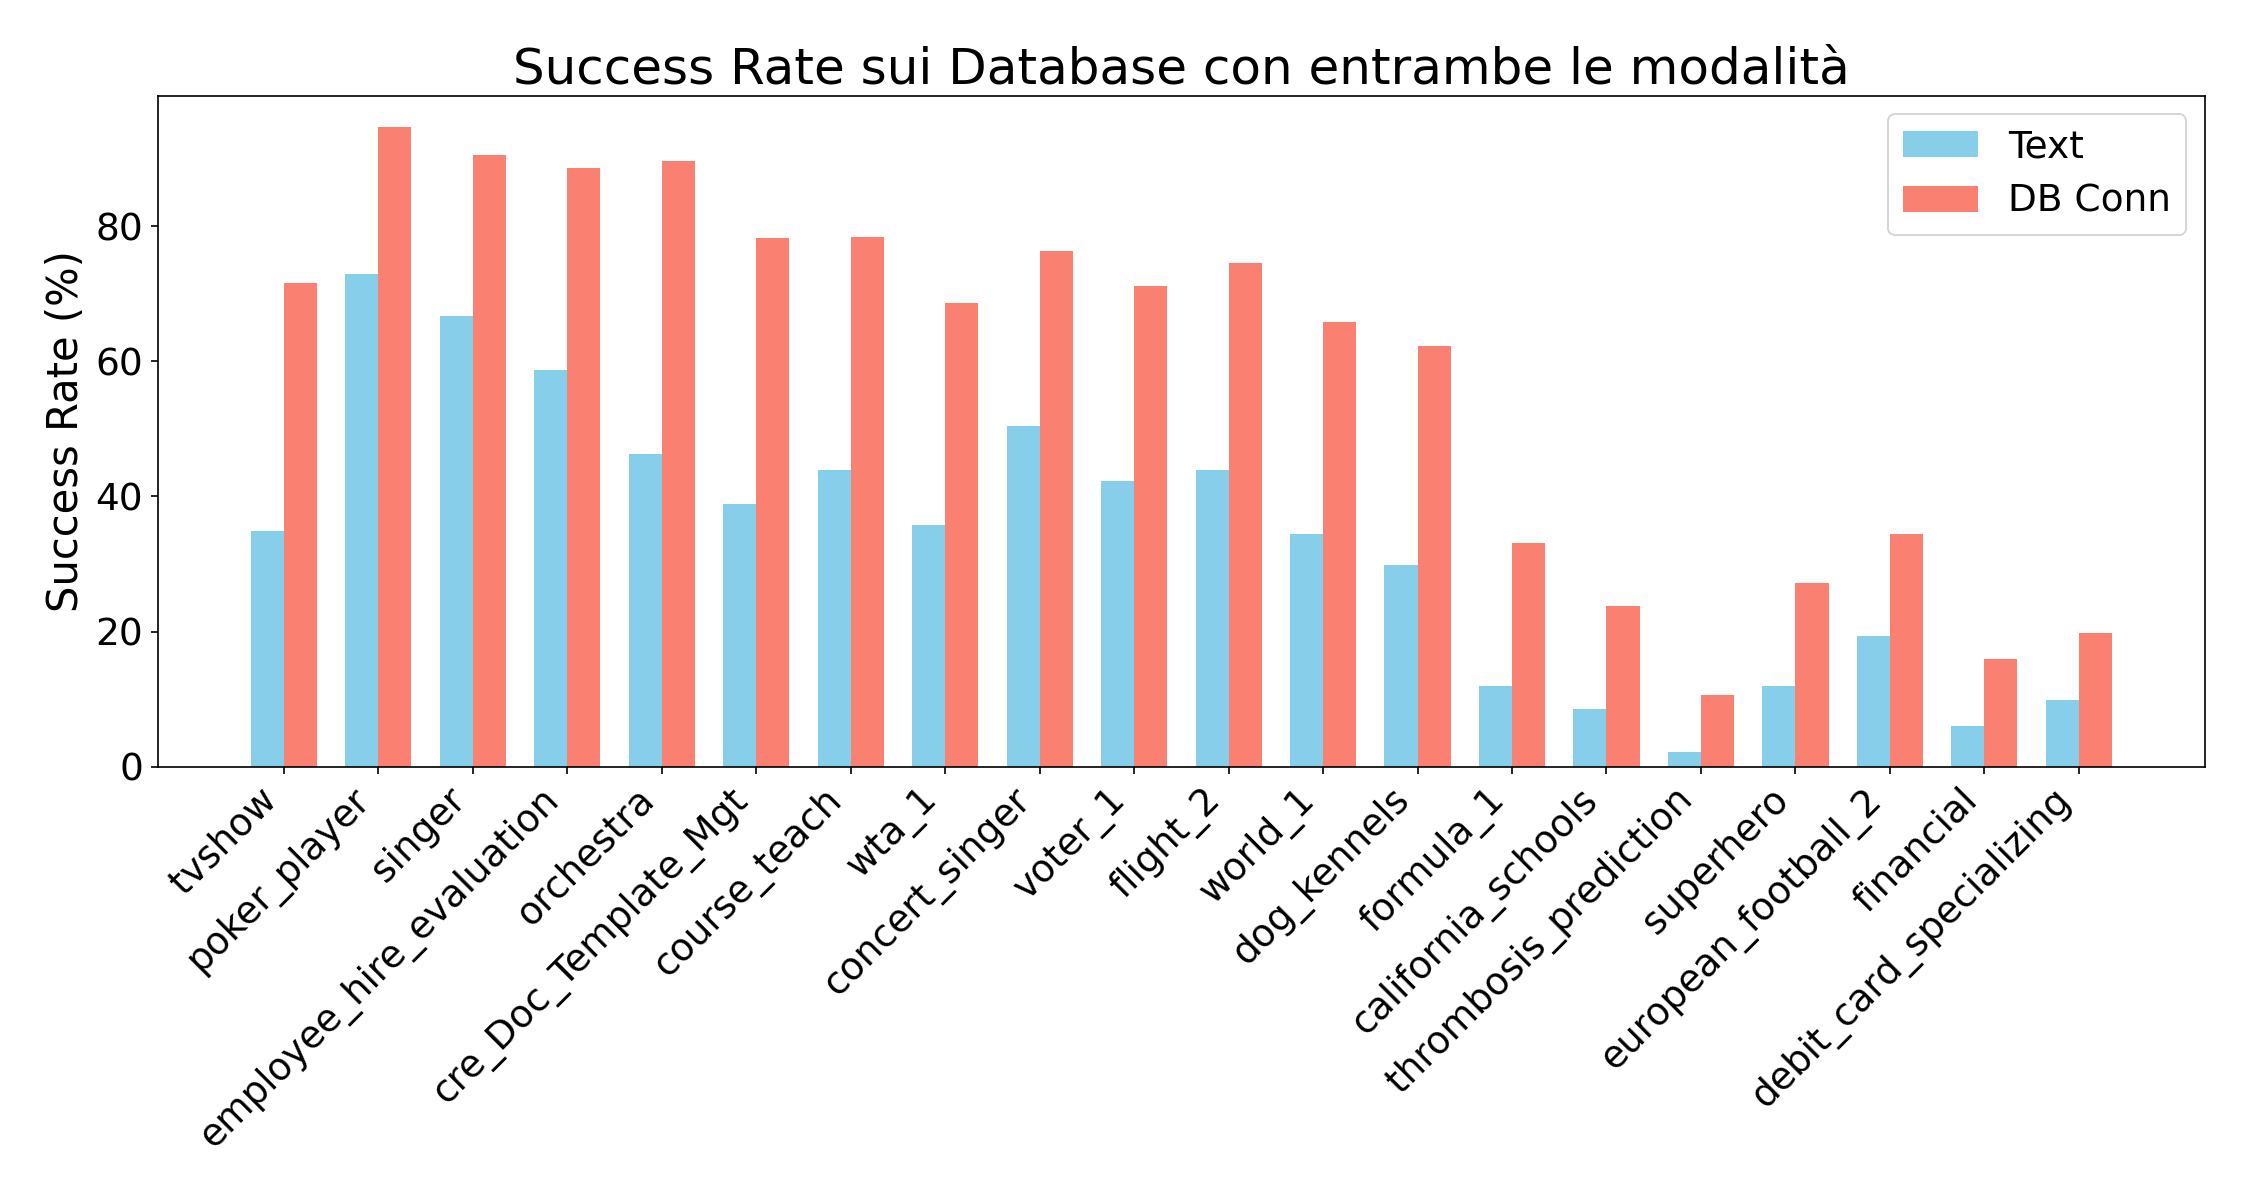
\includegraphics[width=0.95\textwidth]{immagini/charts/db_successes.png}
  \caption{Numero di query risolte correttamente per database e per modalità.}
  \label{fig:db-successes}
\end{figure}

\subsection{Analisi Comparativa del Comportamento dei
Modelli}\label{analisi-comparativa-del-comportamento-dei-modelli}

Al fine di comprendere l'efficacia dell'introduzione di una connessione
diretta al DBMS rispetto alla pipeline puramente testuale, è necessario
analizzare nel dettaglio il comportamento di ciascun modello all'interno
dei diversi domini operativi (Tabelle \ref{tab:status_gpt4o}--\ref{tab:status_qwen3}). La disamina che
segue mappa le reazioni delle architetture neurali strutturando il
confronto lungo tre direttrici fondamentali: l'efficienza temporale, il
numero di tentativi di raffinamento iterativo e l'anatomia dei
fallimenti generativi (ripartiti in errori di sintassi, eccezioni a
runtime e incongruenze semantiche).

L'introduzione della modalità \texttt{db\_conn}, la quale prevede cicli
iterativi di feedback basati sui messaggi d'errore nativi del DBMS,
comporta una mutazione dei tempi complessivi di elaborazione.

I modelli \texttt{Codestral} e \texttt{Qwen3-Coder-Next} dimostrano la
migliore ottimizzazione dei tempi nella modalità assistita (Tabelle
\ref{tab:status_codestral} e \ref{tab:status_qwen3}). In particolare, \texttt{Qwen3-Coder-Next} fa registrare
un tempo medio globale in modalità \texttt{db\_conn} di soli \(11,15\)
secondi (a fronte dei \(5,35\) secondi in modalità \texttt{text}),
contenendo il decremento prestazionale temporale (\(\Delta\)) a un
sostenuto \(+5,80\) secondi (Tabella \ref{tab:status_qwen3}). \texttt{Codestral} segue a
breve distanza con una latenza media in \texttt{db\_conn} di \(11,35\)
secondi (\(\Delta = +6,09\) s) (Tabella \ref{tab:status_codestral}). Questi dati evidenziano
la capacità di tali architetture open-weight di processare il
contesto aggiuntivo e i feedback del database in modo
rapido, minimizzando l'overhead computazionale del framework.

Al contrario, il picco di latenza computazionale viene registrato da
\texttt{GPT-5-mini}, il quale fa registrare un tempo medio in
\texttt{db\_conn} di ben \(25,05\) secondi, raddoppiando i già elevati
\(11,58\) secondi della modalità \texttt{text} (\(\Delta = +13,47\) s)
(Tabella \ref{tab:status_gpt5mini}). Tale comportamento denota un approccio marcatamente più
verboso o una maggiore complessità computazionale interna durante le
fasi di raffinamento della query, traducendosi in un costo temporale che
potrebbe risultare proibitivo in contesti di produzione in tempo reale.
Anche \texttt{SQLCoder} mostra criticità evidenti, con una media in
\texttt{db\_conn} di \(21,06\) secondi (Tabella \ref{tab:status_sqlcoder}); in questo
scenario, tuttavia, il sovraccarico è giustificato dall'elevato numero di
tentativi effettuati, a differenza del modello commerciale di OpenAI.

Nel database \texttt{california\_schools}, \texttt{GPT-5-mini} evidenzia
una controtendenza di rilievo: il tempo computazionale decresce da
\(32,76\) secondi in modalità \texttt{text} a \(21,16\) secondi in
\texttt{db\_conn} (\(\Delta = -11,60\) s) (Tabella \ref{tab:status_gpt5mini}). Questo caso
limite suggerisce che, in assenza di uno schema informativo reale, il
modello rimanga vincolato in lunghi cicli di generazione di token
esplorativi (allucinazioni di colonne o tabelle), mentre la precisione
fornita dalla connessione diretta al DBMS ne accelera il processo di
convergenza logica. Di contro, nel database \texttt{poker\_player},
quasi tutte le architetture commerciali e avanzate (\texttt{GPT-4o},
\texttt{GPT-5-mini}, \texttt{Qwen3-Coder-Next}) convergono sulla query
corretta entro un intervallo ridotto (tra i \(5\) e i \(9\) secondi
totali in modalità \texttt{db\_conn}) (Tabelle \ref{tab:status_gpt4o}, \ref{tab:status_gpt5mini}, \ref{tab:status_qwen3}),
facendo intuire che la semplicità strutturale sia in grado di ridurre il costo
del ciclo di feedback.

L'analisi del numero medio di tentativi necessari per giungere alla
formulazione finale della query mette in luce la resilienza e la
capacità di interpretazione dell'errore delle diverse intelligenze
artificiali.

\code{Qwen3-Coder-Next} e \code{Codestral} appaiono come i modelli
più diretti ed efficienti. \code{Qwen3-Coder-Next} richiede una media
di appena \(1,68\) tentativi in modalità \texttt{db\_conn} per
concludere la sessione (con un \(\Delta\) rispetto alla modalità
\texttt{text} di soli \(+0,58\) tentativi) (Tabella \ref{tab:status_qwen3}). Questi dati indicano
che, nella maggior parte dei casi, il modello genera la query corretta
alla prima iterazione o necessita di un solo ciclo di correzione per
sanare l'anomalia. \code{Codestral} si attesta su livelli analoghi,
registrando \(1,79\) tentativi medi in modalità \texttt{db\_conn}
(Tabella \ref{tab:status_codestral}).

Sul versante opposto, \code{SQLCoder} mostra il comportamento più
polarizzato, registrando una media globale di \(4,31\) tentativi in
\texttt{db\_conn} (\(\Delta = +3,02\) tentativi rispetto a
\texttt{text}) (Tabella \ref{tab:status_sqlcoder}). Questo dato indica che \code{SQLCoder}
satura quasi regolarmente il tetto massimo di tentativi consentiti
dalla pipeline, incontrando notevoli difficoltà nel comprendere i
messaggi d'errore restituiti dal DBMS. Il modello reitera variazioni
della query senza riuscire a capitalizzare il feedback ricevuto,
rimanendo intrappolato in loop generativi sterili.

Un comportamento peculiare si osserva nel database
\texttt{thrombosis\_prediction}, dove \texttt{GPT-5-mini} mostra un
\(\Delta\) negativo nei tentativi (\(\Delta = -0,50\)): se in modalità
\texttt{text} effettuava in media \(2,44\) tentativi ciechi, in modalità
\texttt{db\_conn} si ferma a \(1,93\) (Tabella \ref{tab:status_gpt5mini}). Tuttavia,
l'incrocio con i dati sul tasso di successo (stabile al \(12,88\%\))
indica anche che il modello interrompe prematuramente l'esplorazione logica o
che i vincoli imposti dal feedback del DBMS lo portano a troncare la
computazione senza esplorare alternative valide. Al contrario, nel
database \texttt{real\_estate\_properties}, \texttt{SQLCoder} raggiunge
un picco di \(5,25\) tentativi medi, traducendosi in un modesto
\(0\%\) di \emph{Success Rate} in modalità \texttt{db\_conn} (Tabella
\ref{tab:status_sqlcoder}). Questo rappresenta il caso paradigmatico di un'architettura che
esaurisce il budget computazionale senza mostrare alcuna sensibilità ai
feedback di errore dello schema.

%%%%%%%%%%%%%%%%%%%%%%%%%%%%%%%%%% model_attempts & model_times %%%%%%%%%%%%%%%%%%%%%%%%%%%%%%%%%%%

\begin{figure}[htbp]
  \centering
  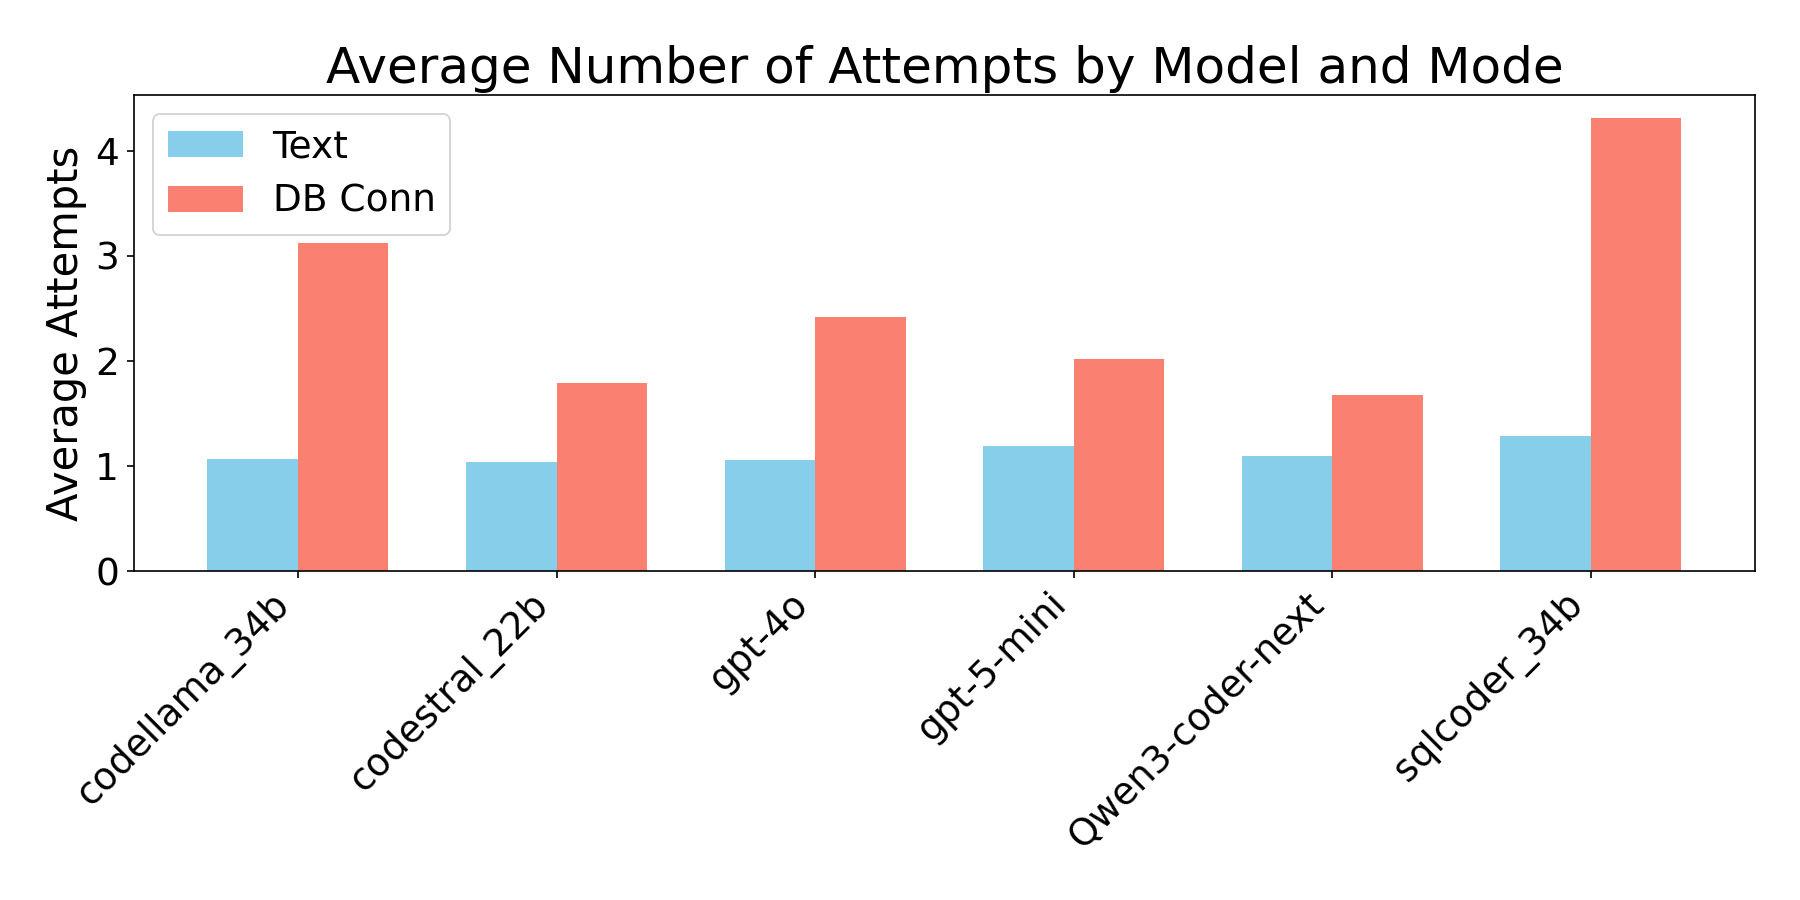
\includegraphics[width=0.95\textwidth]{immagini/charts/model_attempts.png}
  \caption{Numero medio di tentativi e tempo medio di esecuzione per modello.}
  \label{fig:model-attempts-times}
\end{figure}

\begin{figure}[htbp]
  \centering
  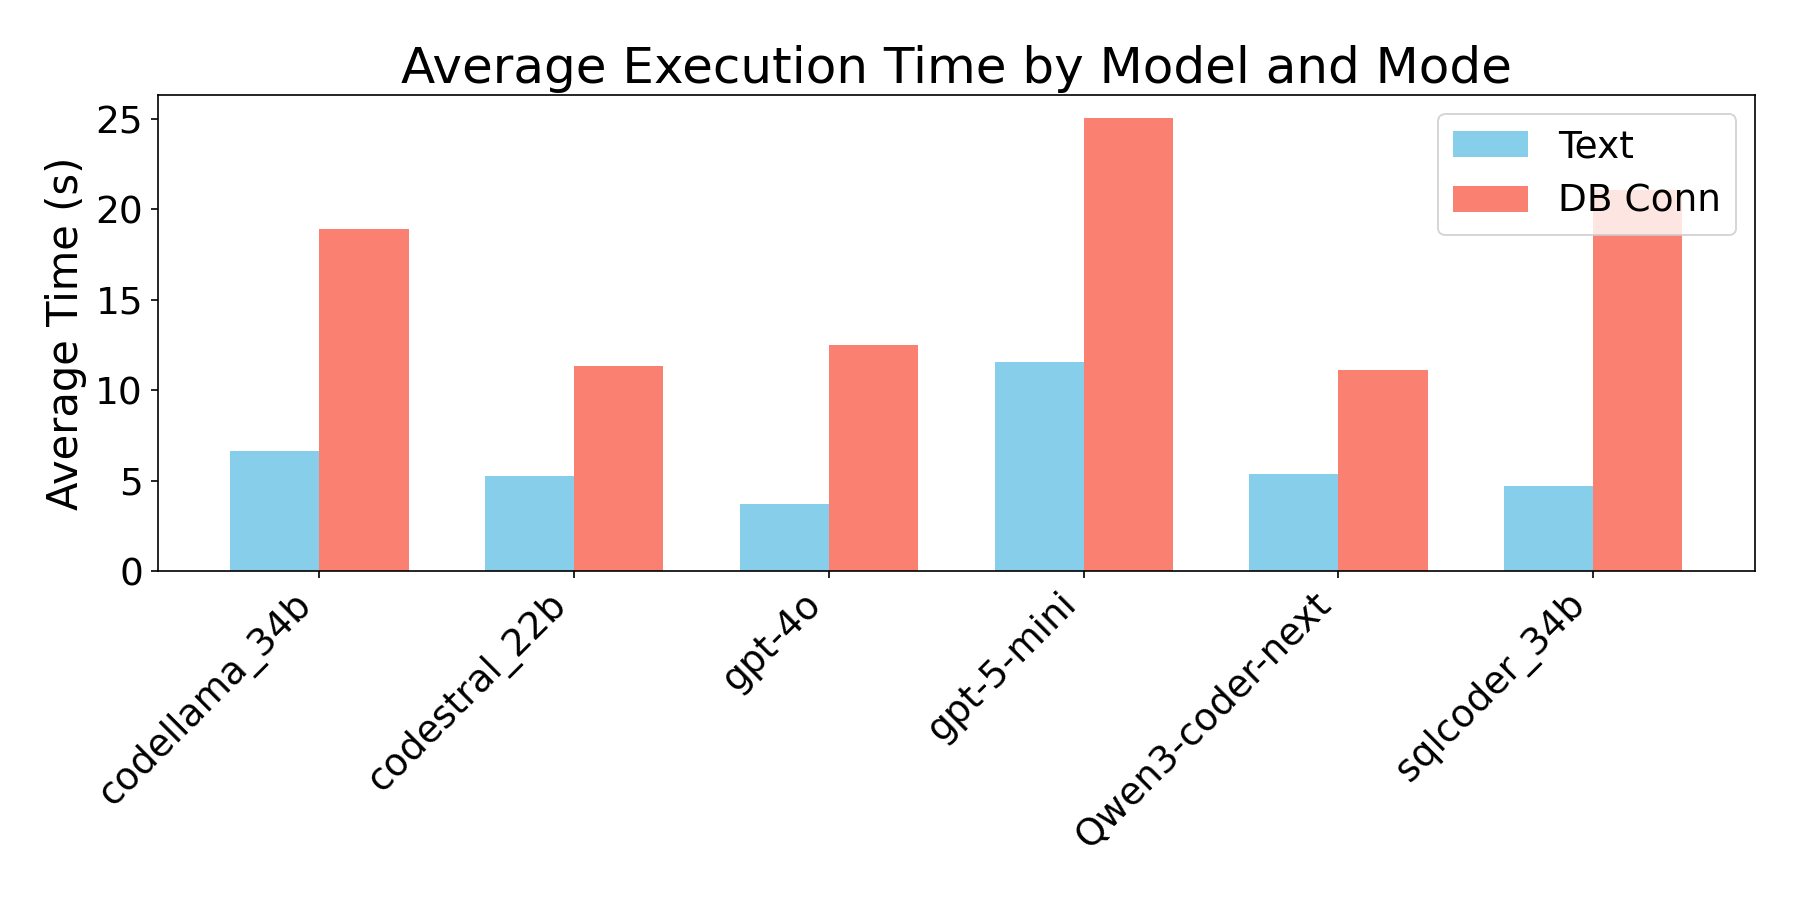
\includegraphics[width=0.95\textwidth]{immagini/charts/model_times.png}
  \caption{Numero medio di tentativi e tempo medio di esecuzione per modello.}
  \label{fig:model-times}
\end{figure}

La categorizzazione dei fallimenti (\texttt{Syntax}, \texttt{Runtime},
\texttt{Incorrect}) permette di mappare la natura profonda dei limiti di
ciascun modello (Tabelle \ref{tab:status_gpt4o}--\ref{tab:status_qwen3}). Un'evidenza macroscopica emerge
immediatamente dall'analisi dei dati: per tutti e sei i modelli
esaminati, gli errori di sintassi pura (\texttt{Syntax}) in modalità
\texttt{db\_conn} sono pari a zero. La pipeline di ingegneria del prompt
e la natura intrinseca dei modelli attuali sono riuscite a rimuovere le anomalie di
parsing elementari in tutte le sessioni di test; la sfida valutativa si sposta interamente sulle
eccezioni a runtime e sugli errori semantici.

Gli errori di runtime, ovvero query sintatticamente valide che
falliscono durante l'esecuzione sul database a causa di identificatori
errati, tabelle inesistenti o join ambigue, variano sensibilmente tra
i modelli. \texttt{GPT-5-mini} e \texttt{Qwen3-Coder-Next} guidano la
classifica della sicurezza esecutiva. \texttt{GPT-5-mini} commette solo
\(38\) errori di runtime globali in modalità \texttt{db\_conn} (a fronte
dei \(2021\) registrati in modalità \texttt{text}), mettendo in luce un
decremento significativo (\(\Delta = -1983\) errori) (Tabella \ref{tab:status_gpt5mini}).
\texttt{Qwen3-Coder-Next} si attesta a soli \(55\) errori di runtime in
\texttt{db\_conn} (\(\Delta = -291\)) (Tabella \ref{tab:status_qwen3}). Questo rivela
l'efficacia euristica del modulo di connessione, che permette a tali
modelli di correggere istantaneamente le sviste di nomenclatura
strutturale dello schema relazionale. Di contro, \texttt{SQLCoder}
fallisce ripetutamente il debugging a runtime, totalizzando \(1016\)
errori in \texttt{db\_conn} (Tabella \ref{tab:status_sqlcoder}). Sebbene riduca i fallimenti
rispetto alla modalità \texttt{text} (\(1712\) errori,
\(\Delta = -696\)), la cifra assoluta rimane critica, testimoniando
l'incapacità del modello di elaborare la natura delle eccezioni SQL (ad
esempio, l'errore \emph{Unknown column} in una clausola \texttt{WHERE}).

Gli errori classificati come \texttt{Incorrect} rappresentano il
fallimento più insidioso nell'interazione Text-to-SQL: la query viene
eseguita dal DBMS senza sollevare eccezioni, ma restituisce un set di
dati errato rispetto ai requisiti logici espressi dall'utente.
L'introduzione della metrica di \emph{Incorrect Rate} consente di
isolare la pura capacità di comprensione semantica del modello,
separandola dalla sua abilità nel generare codice formalmente valido.

Il modello \texttt{GPT-4o} possiede un comportamento antitetico tra le due
modalità (Tabella \ref{tab:status_gpt4o}). In configurazione \texttt{text}, il modello
registra un numero assoluto di errori semantici relativamente basso,
dinamica dovuta esclusivamente all'elevato tasso di fallimenti a runtime
(\(2191\) query bloccate), che riduce in maniera considerevole il campione di query
giunte a esecuzione effettiva. Infatti, laddove la query riesce a essere
eseguita, l'\emph{Incorrect Rate} locale tocca picchi critici (pari al
\(65\%\) in \texttt{california\_schools} e al \(61,54\%\) in
\texttt{superhero}). Nel passaggio alla modalità \texttt{db\_conn},
l'introduzione del contesto strutturato azzera quasi i runtime (crollati
a \(102\)), ma fa traslare gli errori semantici assoluti a \(995\)
(\(\Delta = +910\)) (Tabella \ref{tab:status_gpt4o}).

Al contrario, \texttt{Qwen3-Coder-Next} e \texttt{Codestral} suggeriscono
una discreta robustezza logica, mantenendo l'\emph{Incorrect Rate}
bilanciato tra le due modalità e, in diversi scenari, registrando
persino un incremento della percentuale di query corrette in
\texttt{db\_conn} (ad esempio, \texttt{Qwen3-Coder-Next} riduce
l'incidenza di errore in \texttt{superhero}) (Tabelle \ref{tab:status_codestral} e \ref{tab:status_qwen3}).
\texttt{Qwen3-Coder-Next} si attesta a \(976\) errori semantici in
\texttt{db\_conn} (\(\Delta = +196\) rispetto a \texttt{text}) (Tabella
\ref{tab:status_qwen3}), mentre \texttt{Codestral} ne totalizza \(1040\)
(\(\Delta = +124\)) (Tabella \ref{tab:status_codestral}). Tali dati attestano come questi
modelli specialistici non si limitino a sfruttare lo schema per
risolvere la sintassi, ma ne assimilino i vincoli relazionali per
raffinare la precisione dell'output logico.

Nei database caratterizzati da un'elevata densità informativa e da un
lessico settoriale, si assiste a una massiccia conversione degli errori
a runtime in errori semantici, specialmente nelle architetture di ultima
generazione. Emblematico è il caso di \texttt{GPT-5-mini} sul database
\texttt{toxicology}: gli errori di runtime si azzerano completamente in
modalità \texttt{db\_conn} (rispetto ai \(144\) in \texttt{text}), ma
l'\emph{Incorrect Rate} si attesta stabilmente sul \(100\%\) delle query
eseguite (Tabella \ref{tab:status_gpt5mini}), evidenziando una traslazione totale del
fallimento dalla forma al contenuto logico.

A seguito di un'ispezione approfondita condotta sui log di sistema, è
stato possibile isolare la causa determinante di tale fenomeno,
riscontrabile anche in domini apparentemente meno complessi o con un
contenuto numero di tabelle e colonne (quali
\texttt{real\_estate\_properties}, \texttt{card\_games},
\texttt{thrombosis\_prediction} e \texttt{superhero}). In questi
scenari, la risoluzione del task richiede l'applicazione di filtri
stringenti all'interno della clausola \texttt{WHERE} su attributi di
tipo \texttt{VARCHAR}. Tuttavia, i valori categoriali o testuali esatti
necessari a soddisfare il predicato algebrico non vengono specificati
nella richiesta in linguaggio naturale, né sono desumibili dalla mera
struttura dello schema relazionale. Di conseguenza, i Large Language
Models eseguono ripetuti tentativi alla cieca inserendo stringhe
letterali plausibili ma fattualmente errate. Il DBMS esegue con successo
la query (azzerando i runtime error) ma restituisce un set di dati vuoto
o non conforme a quelli della \emph{gold query}, sancendo il fallimento
semantico della generazione e saturando inutilmente il budget di
raffinamento iterativo.

In conclusione, l'analisi di dettaglio rivela che
\texttt{Qwen3-Coder-Next} e \texttt{Codestral} rappresentano le
soluzioni più bilanciate ed efficienti, in quanto capaci di convergere
rapidamente con ridotti tempi di elaborazione, richiedere un numero
esiguo di iterazioni e mostrare un controllo ottimale sui runtime senza
incrementare in modo anomalo la quota di errori logici. Parallelamente,
i modelli proprietari \texttt{GPT-4o} e \texttt{GPT-5-mini} beneficiano
in modo non indifferente della modalità connessa per abbattere i propri
errori di runtime, i quali nella modalità \texttt{text} ne azzeravano
quasi completamente l'usabilità; tuttavia, queste architetture pagano il
prezzo di un sensibile aumento dei tempi di elaborazione e di una forte
traslazione dei fallimenti verso la dimensione semantica
(\texttt{Incorrect}).

Infine, modelli come \texttt{SQLCoder} e \texttt{CodeLlama}, con
quest'ultimo caratterizzato da un \emph{Success Rate} generale ancorato
al \(34,81\%\) in modalità \texttt{db\_conn} (Tabella \ref{tab:status_codellama}), 
appaiono inadatti a contesti di interazione dinamica con il DBMS,
poiché faticano a interpretare correttamente i messaggi di errore
restituiti dal sistema e finiscono per saturare tutti i tentativi
disponibili senza mostrare una reale capacità di auto-correzione.

%%%%%%%%%%%%%%%%%%%%%%%%%%%%%%%%%% model_comparison %%%%%%%%%%%%%%%%%%%%%%%%%%%%%%%%%%%

\begin{figure}[htbp]
  \centering
  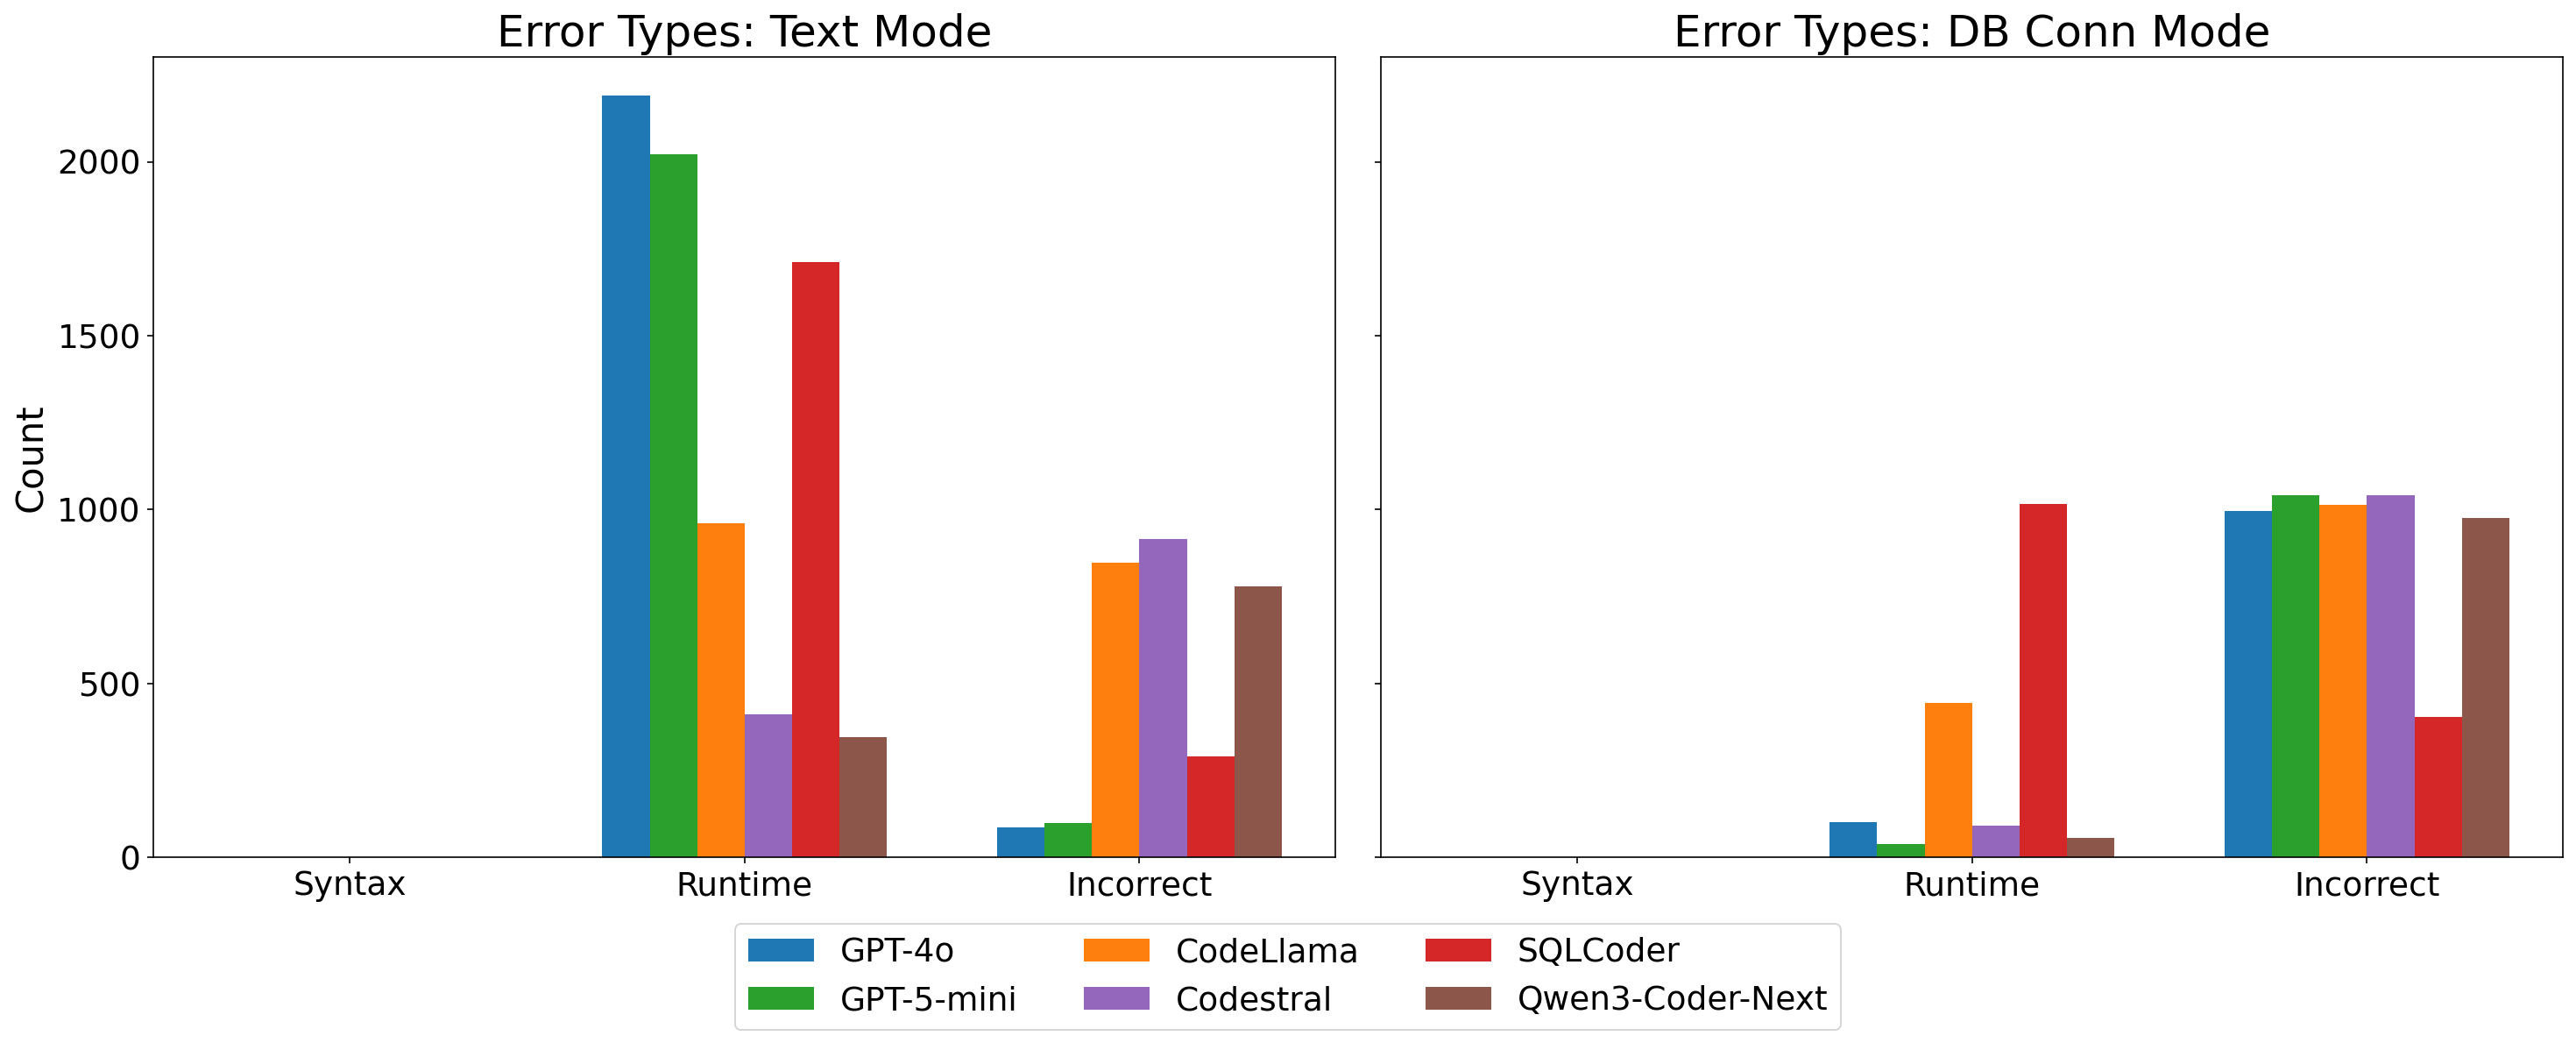
\includegraphics[width=0.95\textwidth]{immagini/charts/error_comparison.png}
  \caption{Confronto delle tipologie di errore riscontrate nei diversi modelli.}
  \label{fig:error-comparison}
\end{figure}

\subsection{Analisi Inferenziale e Studio delle Correlazioni
Statistiche}\label{analisi-inferenziale-e-studio-delle-correlazioni-statistiche}

L'analisi dei coefficienti di correlazione lineare di Pearson
(\(\rho\)), deputato a misurare l'intensità delle relazioni lineari, e
di correlazione per ranghi di Spearman (\(r_s\)), orientato a
intercettare relazioni monotoniche anche non lineari, consente di
caratterizzare l'impatto reale di due variabili esogene sulla
probabilità di successo del codice SQL generato (codificato come
variabile binaria \(Y \in \{0,1\}\), dove \(1\) indica il successo e
\(0\) il fallimento). Le variabili d'indagine considerate sono il numero
di tentativi di raffinamento (\emph{attempts}) impiegati
dall'orchestrazione e l'indice di complessità normalizzato del database
(\emph{complexity score}).

I dati estratti relativi alla correlazione tra il numero di iterazioni e
l'esito della generazione mostrano trend consistenti tra le sei
architetture esaminate (\texttt{CodeLlama}, \texttt{Codestral},
\texttt{GPT-4o}, \texttt{GPT-5-mini}, \texttt{Qwen3-Coder-Next},
\texttt{SQLCoder}) (Tabelle \ref{tab:attempts_gpt4o}--\ref{tab:attempts_qwen3}), svelando dinamiche cruciali
sulla capacità delle singole strutture di capitalizzare il feedback di
esecuzione del database (\texttt{db\_conn}) rispetto al contesto
puramente testuale (\texttt{text}).

Sotto il profilo metodologico, data la codifica binaria della variabile
target, una correlazione negativa indica che l'aumento dei
tentativi di raffinamento è associato a una contrazione sistematica
della probabilità di successo. Questo segno, ampiamente diffuso nel
dataset, indica come i modelli tendano a concentrare l'efficacia
risolutiva nelle primissime iterazioni. Al contrario, il prolungarsi
della sessione verso i limiti superiori di raffinamento non produce
benefici incrementali, mostrando che l'algoritmo tende a rimanere
vincolato in loop generativi sterili o a divergere progressivamente
dall'intento semantico originario.

I modelli \texttt{GPT-4o} e \texttt{CodeLlama} (quest'ultimo in contesti
specifici quali il database \texttt{battle\_death}) rivelano
coefficienti di correlazione negativi robusti e statisticamente
significativi (\(p\text{-value} < 0,05\)) (Tabelle \ref{tab:attempts_gpt4o} e \ref{tab:attempts_codellama}). In
particolare, per \texttt{GPT-4o}, la convergenza verso una correlazione
negativa marcata nella configurazione \texttt{db\_conn} certifica che,
sebbene il sistema sia predisposto per l'auto-correzione, l'esaurimento
dei tentativi si traduce in un decremento della probabilità di successo;
se l'errore non viene sanato immediatamente nel primo ciclo di feedback,
i messaggi del DBMS nelle iterazioni successive faticano a riallineare
la query, agendo talvolta come rumore informativo che induce il modello
a tentare variazioni strutturali non conformi.

Al contrario, \texttt{Codestral} e \texttt{Qwen3-Coder-Next} evidenziano
dinamiche parzialmente differenti in scenari localizzati. Nel database
\texttt{battle\_death}, ad esempio, presentano una correlazione
debolmente positiva, sebbene non statisticamente rilevante
(\(p\text{-value} > 0,05\)), con un coefficiente di Pearson pari a
\(+0,1155\) per \texttt{Codestral} (Tabella \ref{tab:attempts_codestral}) e a \(+0,1615\) per
\texttt{Qwen3-Coder-Next} (Tabella \ref{tab:attempts_qwen3}). Tale lieve inversione di
tendenza indica una sporadica capacità di queste architetture di
beneficiare dei tentativi avanzati per convertire un fallimento iniziale
in successo, sebbene il dato non trovi una spinta statistica sufficiente
a scardinare il trend negativo globale.

In questo scenario, il delta computazionale individua la misura in cui
la connessione dinamica al database modifichi l'efficacia dei tentativi
rispetto al mero ragionamento statico sulle istruzioni DDL. In modelli
verticali come \texttt{SQLCoder}, si osserva un comportamento
asimmetrico: nel dominio \texttt{battle\_death} il modello registra una
correlazione negativa significativa in modalità \texttt{db\_conn}
(\(\rho = -0,5375\)) che si azzera nel passaggio alla modalità
\texttt{text} a causa della mancanza di dati validi (valori
contrassegnati come \emph{Non Rilevabili} o assenti) (Tabella \ref{tab:attempts_sqlcoder}).
In tale scostamento si riscontra la dipendenza di SQLCoder dal feedback d’errore interattivo
per tentare una qualsiasi forma di
movimento nella pipeline, pur confermando che l'accumulo di iterazioni
deteriora linearmente l'accuratezza finale.

Il modello \texttt{GPT-5-mini} mostra un andamento emblematico su
database ridotti o specifici (Tabella \ref{tab:attempts_gpt5mini}), dove l'assenza di
correlazione misurabile o valori prossimi allo zero indicano che
l'architettura soffre di un'alta varianza su schemi compatti, in cui un
singolo fallimento iniziale tende a compromettere irrevocabilmente l'evoluzione
statistica dei tentativi successivi senza mostrare un pattern di declino
o crescita lineare definito.

Esaminando i dati aggregati sulla correlazione tra la complessità (sia
della query che dello schema) e il tasso di successo (Tabelle
\ref{tab:complexity_gpt4o}--\ref{tab:complexity_qwen3}), emergono macro-tendenze fondamentali che accomunano
l'intero corpus di test.

La prima evidenza è rappresentata dalla correlazione negativa
generalizzata: la quasi totalità dei coefficienti aggregati di Pearson e
Spearman presenta valori negativi significativi, supportati da un
\(p\text{-value}\) matematicamente prossimo allo zero (con ordini di
grandezza compresi tra \(10^{-15}\) e \(10^{-49}\)). I \(p\text{-value}\) 
molto bassi indicano una forte evidenza statistica di associazione nel 
campione analizzato, pur con le cautele dovute alla dipendenza tra osservazioni 
appartenenti allo stesso database e allo stesso modello. Tale dato mette in luce il fatto
che all'aumentare della complessità della richiesta o della densità dello schema 
relazionale, la probabilità di successo dei modelli diminuisce costantemente.

Dall'analisi dei valori medi emerge inoltre il vantaggio strutturale
della modalità \texttt{db\_conn} rispetto a quella \texttt{text}. La
complessità dello schema mostra una correlazione negativa più marcata nella modalità connessa;
\texttt{CodeLlama}, a titolo esemplificativo, registra un coefficiente
di \(-0,2928\) contro il \(-0,2267\) della modalità testuale (Tabella
\ref{tab:complexity_codellama}). Tale dinamica indica che la complessità dello schema penalizza
maggiormente i modelli quando questi sono vincolati a una connessione
database reale, un fenomeno riconducibile alla rigidità sintattica
richiesta per l'esecuzione diretta sul DBMS rispetto alla maggiore
tolleranza tipica del parsing testuale astratto.

Si rileva, infine, un notevole allineamento tra i coefficienti di
Pearson e Spearman, i quali seguono traiettorie quasi identiche. Questa
convergenza attesta la robustezza statistica del dato, indicando che
il declino delle performance non è causato da anomalie isolate o
outliers, ma rappresenta un trend monotonico e strutturale
intrinseco al comportamento dei modelli.

I modelli esaminati non reagiscono in modo uniforme ai fattori di
complessità, ma possono essere ripartiti in tre distinte classi di
resilienza:

\begin{enumerate}
\def\labelenumi{\arabic{enumi}.}
\item
  \textbf{Architetture Specialistiche di Vecchia Generazione
  (\texttt{CodeLlama}, \texttt{SQLCoder}):} \texttt{CodeLlama} mostra la
  sensibilità più severa e lineare alla complessità dello schema,
  registrando un coefficiente di Pearson in modalità \texttt{db\_conn}
  pari a \(-0,2928\) nella media delle colonne (Tabella \ref{tab:complexity_codellama}). Il
  modello manifesta criticità evidenti nell'orchestrazione di schemi
  estesi e mantiene un trend rigidamente negativo prossimo a \(-0,17\)
  in entrambe le modalità operative. \texttt{SQLCoder} esibisce un
  comportamento affine, sebbene con una penalizzazione leggermente
  inferiore sulla complessità dello schema (\(\rho = -0,1798\) in
  \texttt{db\_conn}) (Tabella \ref{tab:complexity_sqlcoder}). In questo caso, il delta tra le
  modalità \texttt{db\_conn} e \texttt{text} si attesta a un marginale
  \(-0,0058\), evidenziando come il modello risenta della complessità
  architetturale a prescindere dall'interfaccia di interazione adottata.
\item
  \textbf{Classe Intermedia ad Alte Prestazioni (\texttt{Codestral},
  \texttt{Qwen3-Coder-Next}):} \texttt{Codestral} registra una delle
  correlazioni negative più marcate sulla complessità complessiva della
  query, con un valore di Spearman in modalità \texttt{db\_conn} pari a
  \(-0,2135\) (Tabella \ref{tab:complexity_codestral}). Questo dato denota che, nonostante si
  tratti di un'architettura nativa per il codice, le richieste
  strutturalmente pesanti ne minano profondamente l'accuratezza. Al
  contrario, \texttt{Qwen3-Coder-Next} dimostra un comportamento
  peculiare: l'impatto negativo della complessità dello schema in
  modalità \texttt{text} (\(-0,2186\)) è superiore rispetto alla
  modalità \texttt{db\_conn} (\(-0,1907\)), generando un delta positivo
  di \(+0,0279\) (Tabella \ref{tab:complexity_qwen3}). Tale inversione suggerisce una
  spiccata capacità del modello di beneficiare della connessione al
  database attivo per validare e gestire gli schemi complessi.
\item
  \textbf{Modelli di Frontiera e Ragionamento (\texttt{GPT-4o},
  \texttt{GPT-5-mini}):} \texttt{GPT-4o} si dimostra l'architettura più
  resiliente alla complessità in configurazione testuale; nella
  valutazione sul totale del modello in modalità \texttt{text}, registra
  un coefficiente di Pearson pressoché nullo (\(+0,0153\)) associato a
  un \(p\text{-value}\) non significativo di \(0,4530\) (Tabella \ref{tab:complexity_gpt4o}).
  Di conseguenza, \texttt{GPT-4o} è l'unico modello le cui performance
  su testo non sono linearmente influenzate dalla complessità della
  query, sebbene il passaggio alla modalità \texttt{db\_conn} riporti la
  correlazione a un valore negativamente significativo (\(-0,1909\)),
  evidenziando l'impatto dei vincoli reali del DBMS. \texttt{GPT-5-mini}
  segue l'andamento del predecessore mostrando una forte contraction
  dell'impatto della complessità in modalità \texttt{text}
  (\(\rho = -0,0582\)), ma palesa comunque una fragilità marcata quando
  si scontra con la complessità strutturale dello schema in modalità
  \texttt{db\_conn}, dove il valore di Pearson per la media delle
  colonne scende a \(-0,1682\) (Tabella \ref{tab:complexity_gpt5mini}).
\end{enumerate}

%%%%%%%%%%%%%%%%%%%%%%%%%%%%%%%%%% correlation_deltas %%%%%%%%%%%%%%%%%%%%%%%%%%%%%%%%%%%

\begin{figure}[htbp]
  \centering
  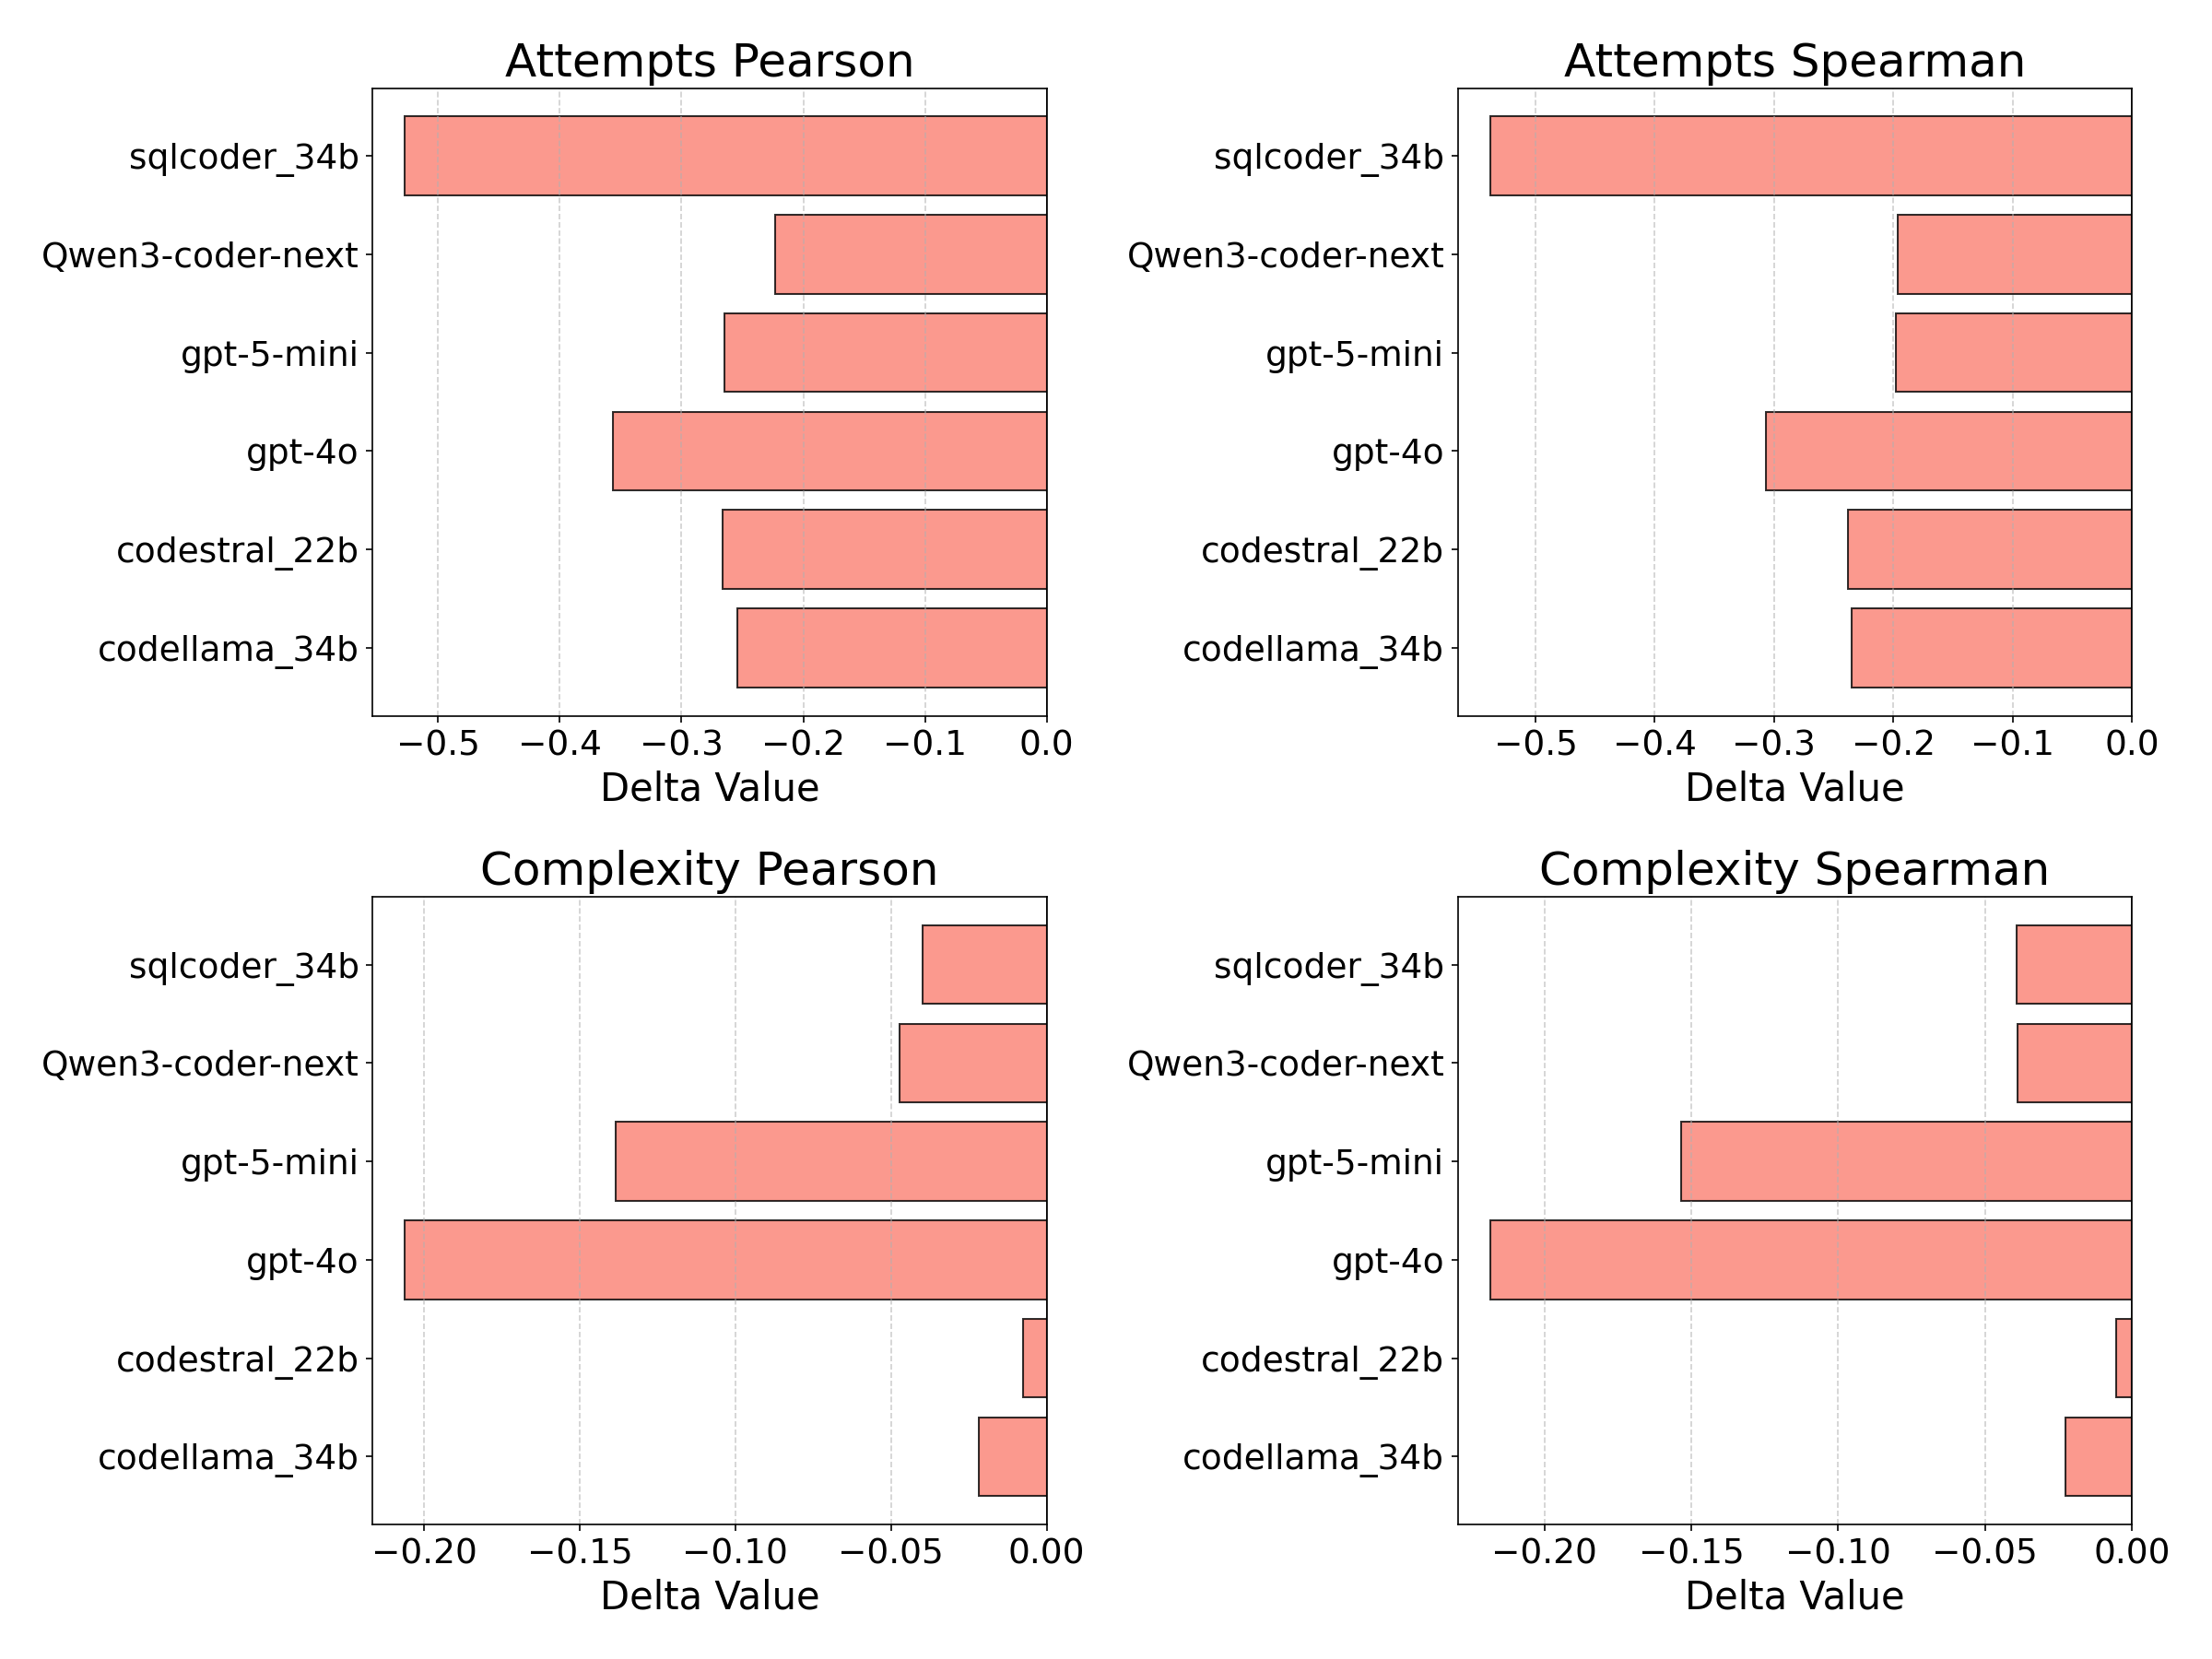
\includegraphics[width=0.95\textwidth]{immagini/charts/correlation_deltas.png}
  \caption{Variazione delle correlazioni tra complessità del database e metriche sperimentali.}
  \label{fig:correlation-deltas}
\end{figure}

La disamina dei singoli database evidenzia dinamiche locali che deviano
dal trend globale, offrendo significativi spunti analitici.

Una prima evidenza è rappresentata dai domini definiti \emph{``Killer
Database''}, quali \texttt{dog\_kennels}, \texttt{world\_1},
\texttt{toxicology} e \texttt{codebase\_community}. In questi contesti,
la totalità dei modelli mostra una correlazione negativa solida e
statisticamente convalidata. Nel database \texttt{dog\_kennels}, ad
esempio, i coefficienti oscillano costantemente tra \(-0,25\) e
\(-0,41\), a dimostrazione del fatto che tali schemi e le relative query
costituiscono il principale collo di bottiglia per l'attuale tecnologia
Text-to-SQL.

Al contrario, in contesti specifici si assiste al fenomeno
controintuitivo delle correlazioni positive anomale, come nei
casi di \texttt{poker\_player}, \texttt{employee\_hire\_evaluation} e
\texttt{cre\_Doc\_Template\_Mgt}. All'interno di \texttt{poker\_player},
\texttt{CodeLlama} registra un coefficiente di Pearson in modalità
\texttt{db\_conn} pari a \(+0,3549\) e \texttt{SQLCoder} raggiunge
\(+0,4155\), mentre \texttt{employee\_hire\_evaluation} mostra in
\texttt{CodeLlama} un valore di \(+0,3753\) in modalità \texttt{text}.
Sotto il profilo tecnico, una correlazione positiva implica che
all'aumentare della complessità i modelli abbiano ottenuto un tasso di
successo superiore. Tale paradosso si ipotizza possa essere causato dalla struttura dei
dati di test: nei database menzionati, le query catalogate come ad alta
complessità presentano pattern sintattici ricorrenti, funzioni di
aggregazione standardizzate o clausole di \texttt{JOIN} obbligate su
chiavi esplicite su cui i modelli potrebbero avere eseguito un overfitting
in fase di addestramento. Viceversa, le richieste classificate come
semplici esibiscono frequenti ambiguità linguistiche nel testo naturale
che inducono i modelli in errore.

Un ulteriore caso limite è rappresentato da \texttt{voter\_1} in
\texttt{GPT-4o}, dove si registra una elevata polarizzazione tra le due
modalità operative: il modello mostra una correlazione negativa in
\texttt{db\_conn} (\(-0,3434\)) a fronte di una correlazione fortemente
positiva in modalità \texttt{text} (\(+0,7447\) con un
\(p\text{-value}\) di \(0,0014\)). Tale comportamento indica che il
modello genera query complesse che testualmente risultano coerenti e
rigorose, giustificando l'alta correlazione su testo, ma che
all'atto pratico falliscono l'esecuzione sul database reale a causa di
disallineamenti di nomenclatura o vincoli di schema non intercettati.

Infine, per i modelli commerciali (\texttt{GPT-4o} e \texttt{GPT-5-mini}), 
si rileva la presenza di coefficienti contrassegnati come
\emph{Non Rilevabili} (ND), circostanza ricorrente su database quali
\texttt{museum\_visit}, \texttt{network\_1} e \texttt{orchestra}. Questa
condizione si verifica quando il tasso di successo del modello nel
database specifico è pari al \(100\%\) o allo \(0\%\) su tutti i livelli
di complessità. Venendo a mancare la varianza nei risultati a causa
della costanza degli esiti, l'algoritmo computazionale azzera il
denominatore nella formula della covarianza, producendo una divisione
per zero che rende formalmente impossibile determinare la correlazione
statistica.

\subsection{Conclusioni dell'Analisi}\label{conclusioni-dellanalisi}

In conclusione, l'impianto sperimentale strutturato attorno al modulo
\texttt{summarize\_models.py} ha permesso di mappare
i confini operativi del sistema con tecnologia Text-to-SQL di
fronte alla complessità dei dati. L'analisi inferenziale condotta
tramite i coefficienti di Pearson e Spearman ha consentito di individuare la presenza
di alcuni trend negativi strutturali e generalizzati: la densità degli
schemi relazionali e la complessità intrinseca delle query rappresentano
i principali fattori esogeni di degradazione delle performance
predittive.

Tuttavia, i dati di test evidenziano come l'introduzione di
un'architettura basata su connessione interattiva al database
(\texttt{db\_conn}) costituisca una strategia di mitigazione
determinante. Sebbene tale modalità imponga un inevitabile
overhead in termini di latenza temporale e richieda cicli di
feedback iterativi, essa azzera di fatto gli errori di sintassi pura e
abbatte in modo significativo le eccezioni a runtime, offrendo ai
modelli una consapevolezza contestuale superiore, altrimenti preclusa
nella configurazione statica su prompt testuale (\texttt{text}).

La disamina empirica delinea una sorta di gerarchia tra i
modelli: mentre le architetture open-weight specialistiche come
\texttt{Qwen3-Coder-Next} e \texttt{Codestral} mostrano un
bilanciamento tra tempi di computazione, accuratezza logica e
interpretazione del feedback di errore, i modelli proprietari di
frontiera (\texttt{GPT-4o} e \texttt{GPT-5-mini}) massimizzano
l'abbattimento dei runtime a prezzo di una marcata traslazione dei
fallimenti verso la dimensione semantica (\texttt{Incorrect}). Al
contrario, le soluzioni di precedente generazione palesano una
sostanziale inidoneità ai contesti dinamici, saturando i tentativi
disponibili senza mostrare una reale capacità di auto-correzione. I
risultati ottenuti non solo validano l'efficacia metodologica del
framework sviluppato, ma forniscono coordinate empiriche fondamentali
per il futuro design di pipeline RAG e agenti autonomi applicati
a sistemi di gestione di database relazionali complessi.
